\section{Prediction Models}
This next chapter describes the Long Short-Term Memory and Auto-Regressive Integrated Moving Average model in detail and what the important topics are when building and training models.
\subsection{Long Short-Term Memory}
The main focus of this thesis, the LSTM, is described in this section in more detail.
The description includes the theoretical background to understanding the basics of LSTMs as well as the practical aspects of building and training an LSTM model.
\subsubsection{Theory \& Background}
\paragraph{Neural Networks}
Neural Networks are a form of machine learning models.
The idea behind them is that they mimic a human brain.
Every neural network is made up of single neurons in different layers; each neuron connects to each neuron of the next layer.
There are three types of neurons: input, output and hidden.
Input neurons get the data into the network, output neurons provide the results and hidden neurons modify the data on the way between the input and output.
The value of a neuron is the weighted sum of all neurons in the previous layer and for each neuron the weights are different.
These weights are the central part that the training is modifying.
This weighted sum is then mapped to a function to calculate the output; one example for such a function would be the Sigmoid function \cite[p. 11]{DeepLearningBook}.

A neural network learns by getting fed input data and after starting with random weights and therefore random outputs, the model checks if the output is correct.
With a function, it then tries to change the weights of the neurons to get closer to the correct output.
After feeding the network with enough data, the function that describes the behaviour of the model should converge on a local minimum.
There exist multiple different functions to calculate the weights; one example is gradient descent \cite[Ch. 10.5.a]{RnnDesign}.
A loss function judges the quality of the predictions, which the optimization function tries to make as small as possible, finding a local minimum.
One loss function that authors use often is the \textit{Mean Squared Error}.
Section \ref{training} closer elaborates on the training of neural networks.

The previously described behaviour is the essential function of a neural network, but there are multiple versions of neural networks, including Recurrent Neural Networks closer described in the next paragraph.

\paragraph{Recurrent Neural Networks}
\begin{figure}[h]
	\centering
	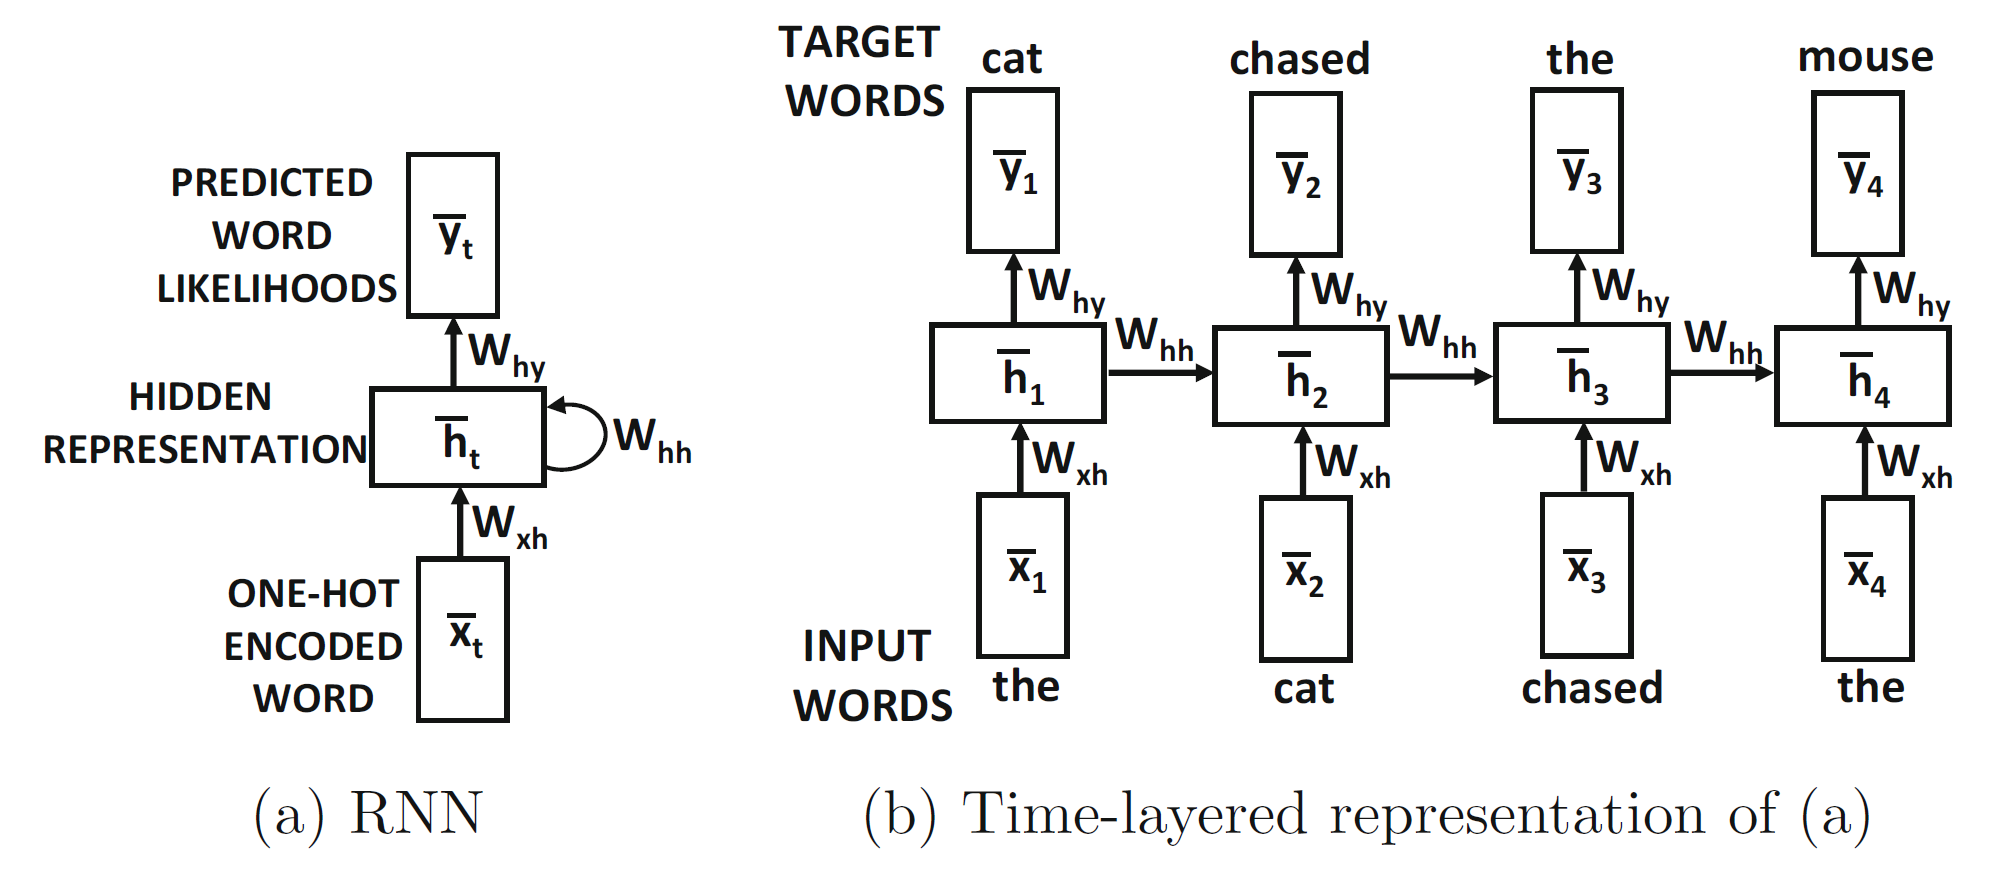
\includegraphics[width=0.7\linewidth]{Pictures/RNN_Structure}
	\caption{The Structure of a RNN a), and its time-layered representation b). \cite[p. 275]{DeepLearningBook}}
	\label{fig:rnnstructure}
\end{figure}
Recurrent Neural Networks (RNN) are also a form of Neural Networks.
However, the difference between a standard Neural Network and an RNN is the preservation of previous outputs, as described in \cite[p. 274ff.]{DeepLearningBook}.
As can be seen in Figure \ref{fig:rnnstructure} a) the RNN has an input $\bar{x}_{t}$, an output $\bar{y}_{t}$ and a number of hidden layers $\bar{h}_{t}$, but what is new in RNN is the self-loop with weights ${W}_{hh}$.
With this loop, information of previously hidden layers is passed to the next instance of the hidden layers when a new input arrives.
This concept gets clearer when viewing Figure \ref{fig:rnnstructure} b) with every new input the output of the previous $\bar{h}_{t-1}$ gets transferred to the next $\bar{h}_{t}$.
The input $\bar{x}_{t}$ for the example in \ref{fig:rnnstructure} b) would be the vector [the, cat, chased, the].
Each of the elements will be an input for a step.
So the RNN would start with the input \textit{the} and use that prediction combined with the next input \textit{cat} for the next prediction continuing with the whole input vector.
As described in \cite[p. 276]{DeepLearningBook} the output vector gets combined with the new input:
\begin{displayquote}
	$\bar{h}_{t} = tanh({W}_{xh}\bar{x}_{t} + {W}_{hh}\bar{h}_{t-1})$
\end{displayquote}                
From this basic version of RNN multiple different more complex variants diverged.
I use one of those variants in this thesis; the LSTM(Long Short-Term Memory) model.

\paragraph{Long Short-Term Memory}\label{LSTM Theory}
The basics of the LSTM are the same with the RNN: it has an input and output and passes its previous output to the next step.
The difference lays in the fact how the LSTM combines the different outputs and inputs and how the model transfers them to the next Neural Network step.
Additionally, to the output, a combining cell-state is also transferred in each step.
This cell-state holds information covering all the steps that were executed previously.
The model updates this state in each step.
The difference of the LSTM to a standard RNN can also be seen inside the cells.
In a basic form, the LSTM is made up of the following:
\begin{itemize}
	\item cell-state ${c}_{t}$:
	\begin{itemize}
		\item forget gate: input is used to decide what to "forget" from the copied cell-state
		\item new cell-state: with the input and the modified cell-state the new state of this cell is calculated.
	\end{itemize}                        
	\item output ${h}_{t}$:
	\begin{itemize}
		\item the input is combined with the new cell-state to determine output. 
	\end{itemize}                        
\end{itemize}
\begin{figure}
	\centering
	\includegraphics[width=.8\linewidth]{"Pictures/LSTM Cell"}
	\caption{Visual representation of an LSTM cell \cite{DBLP:journals/corr/Graves13}}
	\label{fig:lstm}
\end{figure}

The described structure is the basic idea behind LSTMs.
An example of one implementation of an LSTM-cell and how the input, cell-state and output are combined can be seen in Figure \ref{fig:lstm} with the corresponding formulas explained in the following paragraph.

\begin{displayquote}
		\item Input Gate: ${i}_{t}={\sigma}({W}_{xi}{x}_{t} + {W}_{hi}{h}_{t-1} + {W}_{ci}{c}_{t-1} + {b}_{i})$
\end{displayquote}
The input gate determines what information of the input $x_t$ and $h_t$ should be used in the calculation. If a value in the vector $i_t$ is zero the value is not used and if it is one it is used fully.
\begin{displayquote}
		\item Forget Gate:  ${f}_{t}={\sigma}({W}_{xf}{x}_{t} + {W}_{hf}{h}_{t-1} + {W}_{cf}{c}_{t-1} + {b}_{f})$
\end{displayquote}
The forget gate functions similar to the input gate but this gate determines what is "forgotten" from the last cell-state. This can be seen in the formula of the new cell-state $c_t$: ${f}_{t}{c}_{t-1}$.
\begin{displayquote}
		\item Cell-state: ${c}_{t}={f}_{t}{c}_{t-1} + {i}_{t}tanh({W}_{xc}{x}_{t} + {W}_{hc}{h}_{t-1}+{b}_{c})$
\end{displayquote}
The cell-state is created from the combination of the forget gate ${f}_{t}$ with the old cell-state ${c}_{t-1}$ and the input gate $i_t$ combined with the input $x_t$ and the last output $h_{t-1}$.
\begin{displayquote}
		\item Output Gate: ${o}_{t}={\sigma}({W}_{xo}{x}_{t} + {W}_{ho}{h}_{t-1} + {W}_{co}{c}_{t} + {b}_{o})$
		\item Output: ${h}_{t}={o}_{t}tanh({c}_{t})$
\end{displayquote}
Finally the output gate modfies the inputs and the cell-state to produce the actual output of this LSTM step.
The diagram in Figure \ref{fig:lstm} represents one cell in an unrolled version of an LSTM, just like in Figure \ref{fig:rnnstructure} b).

First looking at the inputs in the diagram: ${c}_{t-1}, {h}_{t-1}, {x}_{t}$.
These inputs represent the cell-state (${c}_{t-1}$) and the output (${h}_{t-1}$) of the previous step and the input (${x}_{t}$) to this step.
${c}_{t-1}$ and ${h}_{t-1}$ are both vectors of a length that corresponds to the number of hidden nodes in the LSTM.
The input (${x}_{t}$) to an LSTM is always a 2D-Array; its shape is (time-steps, features).

Let me make a concrete example to understand the LSTM better.
We have a sequence of numbers; [1, 2, 3, 4, 5].
The goal is to predict the 3rd number using the previous two numbers. Then the input array would have a \textit{time-steps} dimension of two, because I have two steps in our sequence (e.g. 1,2) and the \textit{feature} dimension of one, because I have one feature, one time-series.
However, for the calculation at step t, only the element t of the input vector is used.
So the actual input $x_t$ in this example is a vector of shape 1x1 per step.
The input to the first step would be $x_0 = [1]$ and the second step $x_1 = [2]$.
After defining how I shaped the input and output, the form of the weight matrices also becomes apparent.
All internal vectors have the same length as the output vector.
So ${i}_{t}, {f}_{t}, {c}_{t}, {o}_{t}$, all must have the same length as ${h}_{t}$.
All weight matrices $W$ must have the form of $m\times n$ where $n$ is the same dimension as the output vectors and m depends on the vector this matrix is multiplied with.
When using the previous example with the number sequence the input $x_t$ is the shape $1\times 1$ the weight matrices ${W}_{xi},{W}_{xf},{W}_{xo}$ must have the shape $1\times n$, where $n$ is the width of the output.

\subsubsection{Parameters and Architecture of LSTM Models}
This section elaborates closer on the previously described elements of the LSTM and how they can be parameterized and how multiple LSTM layers can be combined.
I used Keras for building the models and use it here as an example of an LSTM implementation.
In Keras the whole LSTM can be customized: activation functions to use, if a bias should be used or not, if weights should be constrained and other values.\footnote{\url{https://keras.io/layers/recurrent/} Accessed: 2019-11-16}
Nevertheless, the underlying architecture of the LSTM can not be changed: input-, output- and forget-gate and the cell-state are part of the LSTM.
However, when staying with the standard LSTM configuration, since I wanted to test a basic LSTM with it standard functions and values.
Then the parameters that one should set are the number of hidden nodes (units) and if the model should return whole result sequence (predictions of each step).
The number of units describes the number of hidden nodes and the length of the output vector.
As described above, it also defines the width of all other vectors and matrices in the LSTM cell and fundamentally set the complexity of the network.
Each LSTM layer can have a different number of hidden nodes.
When combining multiple LSTMs, LSTM layers that come before another LSTM layer have to return the whole sequence of outputs as an input for the next LSTM.
This concept becomes more evident when looking at Figure \ref{fig:singlelstmkeras}: a) shows a single LSTM cell in Keras and its input and output dimension.
It gets an input of shape (batch size, time-steps, features) but the output is in shape (batch size, units).
The output is missing the time-step dimension because only the prediction of the last time-step is returned and not each output of every step.
This is different when looking at the two-layer architecture of the LSTM (Figure \ref{fig:singlelstmkeras} b)).
In this example, after the first layer, all results are returned and put into the next LSTM layer.  
How the batch size factors into the LSTMs and neural networks in general is explained in the Section \ref{training}.          

\begin{figure}
	\centering
	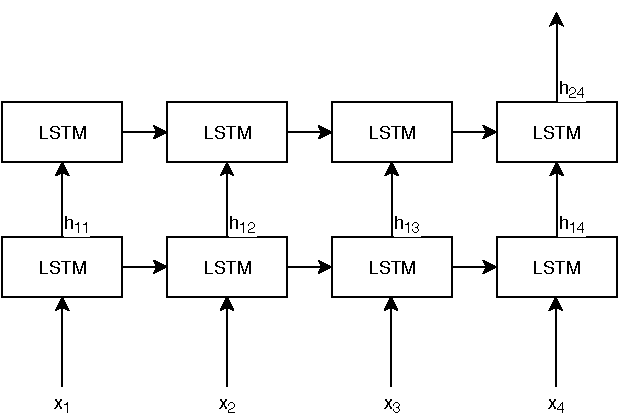
\includegraphics[width=0.7\linewidth]{Pictures/unrolled2layerLSTM}
	\caption{Unrolled version of a two layer LSTM architecture.}
	\label{fig:unrolled2layerlstm}
\end{figure}

To better understand this concept, Figure \ref{fig:unrolled2layerlstm} contains an example of an unrolled two-layer LSTM with four time-steps.
In this example all outputs $h_{11}, h_{12}, h_{13}, h_{14}$ are returned and put into the second LSTM layer.
Moreover, the second layer then only returns the result of $h_{24}$.


\subsubsection{Training an LSTM Model}  \label{training}
The basics of training recurrent neural networks are the same as for all neural networks: the goal is to change the weights of the hidden nodes so that the results get closer to a minimum of the loss function.
As already said, the idea for recurrent neural networks is the same, but it is a more complex problem since one neural network has to change inputs over multiple steps and feeds information forward.
Nevertheless, a close description of how the problem was solved mathematically for recurrent neural networks would be out of scope for this thesis. Because of that, I only give a general description of the ideas behind the optimization of neural networks.
For a closer look at recurrent neural networks, \cite{GradientRecurrent} surveys multiple different approaches modified for recurrent networks.

For the description of how to optimize a neural network, the two main factors are the loss function and the optimizer.
The primary approach is to start with random weights and change the weights after the first result, so the result gets closer to a local minimum of the loss function.
First about the loss function: for this function exist many different approaches, the Keras documentation list multiple approaches\footnote{\url{https://keras.io/losses/} Accessed: 2019-11-16}.
Each of these functions calculates some form of value that describes the quality of a prediction.
One example of the more popular functions is the \textit{Mean Squared Error} function.
It is made up of the simple formula:
\begin{displayquote}
	$MSE=\frac{1}{n}\sum _{i=1}^{n}{\left({Y}_{i}-\hat{{Y}_i}\right)}^{2}$
\end{displayquote}
The Mean Squared Error function is often used to judge the performance of a prediction.
Papers like \cite{deepLearningApproaches} and \cite{8292737} use the MSE or a different form like the Root Mean Squared Error but do not reason why they are using these functions.
However, It is clear that the MSE function is a simple and efficient way of representing the prediction error.

After calculating the loss function, with for example the MSE, the weights need to be changed.
For this, an optimizer is used.
Here are also many examples in the Keras documentation\footnote{\url{https://keras.io/optimizers/} Accessed: 2019-11-16}.
These optimizers use different approaches to change the weights.
One of the frequently used approaches is gradient descent \cite{deepLearningApproaches}:
\begin{displayquote}
	Gradient descent is one of the most commonly used techniques to minimize the loss function.
\end{displayquote}
As one example for an optimizer is the ADAM optimizer \cite{kingma2014adam}, it is also often used in examples for neural networks.
ADAM also uses gradient descent.
The idea behind gradient descent is simple: the gradient of the function is determined and the gradient is followed down to find some local minimum.
When looking at the result of the loss function, the first step is computing the gradient of the loss function.
On these results, the gradient descent updates the weights so that the result of the loss function moves down the gradient.

Keras calculates the gradient via backpropagation, which is also standard practice in machine learning.
Backpropagation is a recursive algorithm to find the steepest gradient of a function.
It starts with the output neurons and looks at the error of each output and how much it needs to be increased or decreased to get closer to a local minimum.
To determine how the output neuron can be changed, the backpropagation algorithm takes the previous layers and its weights into consideration.
When looking at the concrete example in Figure \ref{fig:basic-neural-network}, the formula for describing the one output neuron is as follows:
\begin{displayquote}
	\centering
	$a = a_3\times w_7 + a_4\times w_8 + b$
	\[
	a_5 = \left\{\begin{array}{lr}
	0, & \text{for } a<0\\
	a, & \text{for } 0\leq a\leq 1\\
	1, & \text{for } a>1
	\end{array}\right
	\]
\end{displayquote}
Since the activation of one neuron should not be bigger than 1 or smaller than 0, the function includes the two edge cases. With concrete values the formula looks like this:
\begin{displayquote}
	\centering
	$0.5 = 0.1 \times 0 + 1 \times 0.5 + b$
\end{displayquote}

The bias $b$, in this case, is 0.
Lets say the actual desired output should have been $a_5 = 0.1$.
Three things can be done to decrease the output:
\begin{enumerate}
	\item decrease bias
	\item decrease the weights
	\item change the activations of the previous layer
\end{enumerate}

\begin{figure}
	\centering
	\includegraphics[width=0.7\linewidth]{"Pictures/Basic Neural Network"}
	\caption{Basic example for a neural network with concrete values and linear activation.}
	\label{fig:basic-neural-network}
\end{figure}

The first step, decreasing the bias, would here mean to change it to a negative value to get closer to the output of $a_5 = 0.1$.

Now looking at the weights: here the values of the previous activations $a_4, a_3$ are taken into consideration.
The neuron $a_4$ has activation of 1, so it has the maximum value and the other neuron $a_3$ is at 0.1.
Because of the limitation of the calculation to bigger or equal to 0 and smaller or equal to 1, the maximum value for a neuron is 1 and the minimum 0.
So the weight $w_8$ will be decreased more than $w_7$ because the change in the weight $w_8$ will have more influence on the result of the output because of the higher activation of the neuron $a_4$.

The third step, the change in the activation of the previous neurons, can only be done indirectly, since the activation of the neurons is calculated from previous activations and weights.
How much the neuron activation should change is also in relation to the weights.
That means neuron $a_4$ with weight $w_8$ will be decreased more than the neuron $a_3$ with weight $w_7$, since $w_8$ has the higher weight and more influence on the output because of that.
Now knowing how the activation should be changed, the algorithm does the same for the next layer since the direction of the change in activation $a_3$ and $a_4$ are now known.

The backpropagation is a very time-intensive computation to do.
Because of that, the batch size mentioned in the previous section, \ref{LSTM Theory}, becomes relevant.
Theoretically, in each training step (epoch), the whole data is shown to the network and the backpropagation is performed for each value and gradient descent is then performed on the average of all backpropagations.
When one defines a batch size, the data is split up into multiple sets, each the size previously defined.
Then the network is only shown one batch per training step (epoch).
The result is that the backpropagation and gradient descent is only performed on one batch.
This makes the backpropagation and gradient descent less accurate, but the computation time of the backpropagation is reduced drastically.

\subsection{Auto-Regressive Integrated Moving Average} \label{arima}
The term ARIMA stands for Auto-Regressive Integrated Moving Average; it is a modified version of an ARMA model.
It was introduced in 1970 by Box \& Jenkins \cite{001285997}.
These models are used to predict or simulate time series, but they are no deep learning models like neural networks.
The ARIMA model is also used to predict a time series.
In an ARIMA model three things are combined: An autoregressive model (AR), moving average model (MA) and an integral part (I).
This section gives a short overview of the basics of ARIMA models.
\subsubsection{ARIMA Background}\label{arimaBackground}
When looking at a standard ARIMA model, one can describe the model through three variables: (p,d,q).
As described by \cite{forecasting} the three variables stand for:
\begin{itemize}
	\item p = order of the autoregressive part
	\item d = degree of first differencing involved
	\item q = order of the moving average part
\end{itemize}
The autoregressive model (AR) part of the ARIMA model is using past values of the predicted variable, to model it.
This part is described through the p variable.
What exactly the p stands for becomes clear when looking at the formula of an autoregressive model \cite{forecasting}:
\begin{displayquote}
	$y_t = c+\phi_1y_{t-1}+\phi_2y_{t-2}+...+\phi_p y_{t-p}+\epsilon_t$
\end{displayquote}
So $p$ is just the number of previous values to take into account.
The current variable $y_t$ is described by previous values of itself.
All values are also modified by a parameter $\phi_t$.
Also included in the formula is a constant $c$ and an error $\epsilon_t$ that is just white noise.

When looking at the moving average model (MA), it looks similar to the autoregression model \cite{forecasting}:
\begin{displayquote}
	$y_t = c+\epsilon_t+\theta_1\epsilon_{t-1}+\theta_2\epsilon_{t-2}+...+\theta_q\epsilon_{t-q}$
\end{displayquote}
But here the variable $y_t$ is described through past forecast errors $\epsilon$, also modified with a parameter $\theta_t$.
It is again contained in this formula a constant $c$ and an error $\epsilon_t$ which is also white noise.

Now the third part, the differencing, and how it is defined.
The formula for the differencing in first (a) and second (b) order are \cite{forecasting}:
\begin{samepage}
\begin{displayquote}
	\begin{flushleft}
		$a)$\linebreak
		${y}_{t}^{\prime }=y_t-y_{t-1}$\linebreak
		\linebreak
		$b)$\linebreak
		${y}_{t}^{\prime\prime}=y_t^{\prime}-y_{t-1}^{\prime}$\linebreak
		$=(y_t-y_{t-1})-(y_{t-1}-y_{t-2})$\linebreak
		$=y_t-2y_{t-1}+y_{t-2}$
	\end{flushleft}
\end{displayquote}
\end{samepage}
When differenced once the ${y}_{t}^{\prime}$ is basically the change from one value to the next.
For the ARIMA model, usually only the first and second-order differencing are used.

Putting all three parts together results in the following model:
\begin{displayquote}
	$y_t^{\prime} = c+\phi_1y_{t-1}^{\prime}+...+\phi_p y_{t-p}^{\prime}+\theta_1\epsilon_{t-1}+...+\theta_q\epsilon_{t-q}+\epsilon_t$
\end{displayquote}
In this case $y_t^{\prime}$ could be differenced more than once.        
This is the basic version of an ARIMA model, but what ARIMA is also capable of is predicting seasonal data. 

When working with seasonal data the ARIMA notation changes to (p,d,q) (P,D,Q)m, with m denoting the number of observations per season.
The definition for the (P,Q,D) part is similar to the non-seasonal models, but the shift in the data changes.
So for example, if one uses a p of 1, the term would look like this: $\phi_1y_{t-1}$.
For the seasonal data with 4 observations per season (m=4), a P of 1 would look like this: $\Phi_1y_{t-5}$.
Additionally to the backshift of 1, the data is also shifted back a whole season.
The seasonal terms then get added to the non-seasonal term; that is the seasonal ARIMA model.

\subsubsection{Identifying the Order of ARIMA and its Parameters}
The identification of the order of the single parts of the ARIMA model can either be made manual or automatic.
Since the ARIMA model is not the central part of this thesis, the exact procedure and mathematical background is not explained, but I give a basic overview.
The basic process is displayed in the flowchart Figure \ref{fig:arimaflowchart}.
\begin{figure}
	\centering
	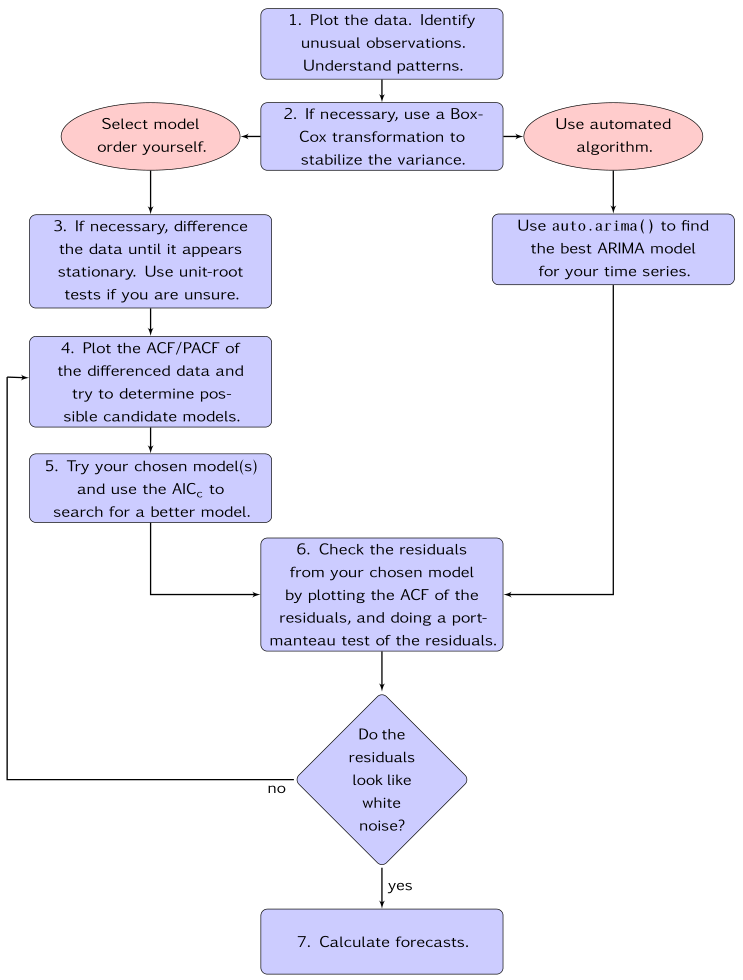
\includegraphics[width=1\linewidth]{Pictures/arimaflowchart}
	\caption{Basic procedure for identifying the order of the ARIMA model.\cite{forecasting}}
	\label{fig:arimaflowchart}
\end{figure}
As already said, the ARIMA is not the main part, so the automatic approach was used for this thesis.
This is described in the Evaluation Section \ref{Eval}   

After the order was selected, the next step is fitting the model to the function.
The actual fitting of the ARIMA model is similar to the training of a neural network.
The parameter $c, \phi , \theta$ are optimized to get the best solution \cite{forecasting}:
\begin{displayquote}
	Once the model order has been identified (i.e., the values of p, d and q), we need to estimate the parameters $c, \phi_1,...,\phi_p, \theta_1,...,\theta_q$. When R estimates the ARIMA model, it uses \textit{maximum likelihood estimation} (MLE). This technique finds the values of the parameters which maximize the probability of obtaining the data that we have observed.
\end{displayquote}
More information about identifying the order and parameter optimizations can be found in \cite{TimeSeriesIntroduction}, \cite{TimeSeriesAnalysis} and \cite{001285997}.

\subsection{Model Setup and Implementation}
This section closer elaborates on the concrete libraries and frameworks that were used to produce the results of this thesis.
\subsubsection{Libraries and Frameworks}
For creating the machine learning models, I chose the library Keras\footnote{\url{https://keras.io/} Accessed: 2019-11-16}.
Keras is a library that enables a user to design, train and use deep machine learning models.
For that, Keras uses one of multiple different machine learning libraries (TensorFlow, Theano or CNTK), TensorFlow in the case of this thesis.

Algorithm \ref{alg_seq_model} shows the basic construction of a machine learning model in Keras.
\begin{algorithm}
	\caption{Creating a sequiental Keras model}
	\label{alg_seq_model}
	\begin{algorithmic}
		\STATE model = Sequential()
		\STATE .
		\STATE .
		\STATE .
		\STATE model.add(Some kind of Keras layer)
		\STATE model.add(Some kind of Keras layer)
		\STATE .
		\STATE .
		\STATE .
		\STATE model.compile(loss=Loss Function, optimizer=Optimizer)
	\end{algorithmic}
\end{algorithm}
The first step is to define a sequential model\footnote{The name sequential here only refers to the sequentially created and stacked layers.}, then add as many layers with their configuration (number of hidden nodes, output shape, activation functions and so forth) as are needed for the model.
The last statement must be the compilation of the model with a loss function and an optimizer.
With this layer architecture, building a model in Keras is easy.
However, what Keras is not helping one with is building a well functioning model.
The different kind of layers, parameters at each layer, the loss function and the optimizer with all its parameters determine the prediction performance.
Finding good values for these parameters and assessing the resulting prediction performance - in comparison with ARIMA - is the goal of this evaluation.
What architecture and parameters were selected is described in Section \ref{archParam}

\subsubsection{LSTM Implementation}
The algorithms are based on an example from the blog \textit{Machinelearningmastery.com}\footnote{\url{https://machinelearningmastery.com/time-series-prediction-lstm-recurrent-neural-networks-python-keras/} Accessed: 2019-11-21}.
The first important function implemented for the LSTM model library is the function for testing for the optimal configuration.
This function uses the Talos framework to test through all defined combinations.
The basic functionality is defined in the algorithm \ref{alg1}.

\begin{algorithm}
	\caption{Test\_for\_optimal\_configuration $inputs:$ $source\_range$, $destination\_range$, $number\_of\_values$, $parameter\_variations$, $number\_of\_repetitions$}
	\label{alg1}
	\begin{algorithmic}
		\STATE test\_folder = create\_test\_result\_folder()
		\FOR{source in source\_range}
		\FOR{destination in destination\_range}
		\STATE data = get\_sub\_data(source, destination, number\_of\_values)
		\STATE data = scale\_values(dataset, 0, 1)
		\STATE training\_values, target\_values = create\_data\_for\_training(data)
		\FOR{repeat in number\_of\_repetitions}
		\STATE start\_talos\_scan(training\_values, target\_values, create\_model\_function, parameter\_variations)
		\ENDFOR
		\STATE move\_test\_data(test\_folder)
		\ENDFOR
		\ENDFOR
	\end{algorithmic} 
\end{algorithm}

At the creation of the library object in the code, one has to define the data that the object is using.
In the first important step of this function, the data is extracted for the source, destination pair and the correct number of most current values.
This data is then scaled correctly between 0 and 1 and from this set, two arrays are created: one with training values and one with the target values.
These values are then put into the Talos scan method, that tries all the previously defined parameter combinations.
The \textit{create\_model\_function} parameter passed to the Talos method is the function that creates the actual model, following the scheme defined in the previous section of how to build a Keras model with added placeholders so that Talos can insert the defined parameters.

The actual method for training one single model is similar to the configuration testing method; that is why I will not add the pseudocode here.
It works the same with some differences.
It just gets a model name it is supposed to train and no parameters it should try, and then it starts the Keras training method.

\subsubsection{PmdARIMA (Automatic ARIMA parameter optimization)}
PmdARIMA is a Python library that provides a possibility to determine the best ARIMA model for predicting a time-series automatically.
For this thesis, I used the traffic of multiple communication pairs.
For this reason, PmdARIMA provides a fast way of generating an ARIMA model without having to analyze every time-series in detail.
The library provides a fast way of generating an ARIMA model to compare the performance of the LSTM predictions.

The optimization does not need many prerequisites.
The parameters previously described in Section \ref{arima} $p,d,q$ and $P,D,Q$ can be set to a specific start value and a maximum that the optimization is not crossing; this can be used to optimize the search for the optimal parameters.
Nevertheless, the optimization can also be started without configuration these values or any other value except one.
The only thing that I had to set is a parameter $m$.
This parameter sets the number of periods one season has, how the m parameter is used was described in section \ref{arimaBackground}.
Examples for this parameter would be:
\begin{itemize}
	\item Quarterly data: m = 4
	\item Monthly data: m = 12
	\item Hourly data: m = 24
\end{itemize}
Important is that the data can contain multiple seasons.
For example, the GÉANT set used in this thesis has 15-minute steps; this leaves multiple possible seasons:
\begin{itemize}
	\item half-hour season: m = 2
	\item one hour season: m = 4
	\item one day season: m = 96
	\item one week season: m = 672
\end{itemize}
I tested all four possibilities.
The test\footnote{Automatically fitted ARIMA model on the communication pair 1 to 11. Using one prediction to test the quality of the model.} showed that m = 4 yielded the model with the best prediction.

The input for the ARIMA model is always an ordered time-series, no matter if it is an automatically fitted ARIMA model or manually fitted one.

An ARIMA model can only ever predict from the last point it was fitted on.
So, for example, if a time series has the values [1,2,3,4,5] and we want to predict the 6th value, the ARIMA model needs to be fitted until the 5.
How long the fitting sequence is, is up to the person fitting the model.
The only thing that cannot be changed is that it has to end with the 5 in this example.
From there, it can make any number of predictions, e.g. the next five steps, but only the first prediction will have a high quality, any prediction after that loses accuracy fast.
What an ARIMA model also does; is that it calculates a confidence interval.
The standard in the PmdARIMA library is a 95\% confidence interval.